\documentclass[10pt]{article}

\usepackage{amsmath}
\usepackage{amsfonts}
\usepackage{graphicx}

\begin{document} 
\title{Resumen de Analisis Numerico}
\author{
        Mateo P. Cetti \\
        Estudiante - Universdad Catolica de Cordoba\\
        Ing Ambrosio Taravella, 6240, \underline{Cordoba, Argentina}
}
\date{\today}

\maketitle

\section{Introduccion}

\subsection{Objetivo del analisis numerico}

El objetivo del analisis numerico es el de enseñarle 
a la computadora a realizar operaciones matematicas complejas.
Se estudian metodos numericos que nos permiten interactuar con la computadora

Antiguamente los metodos numericos eran usados de manera muy limitada por el 
tedioso trabajo de usarlos a mano. Ahora con el auge de las computadoras, 
estos modelos son mas usados y generan mucho mejores resultados.

\subsection{Problematicas}

\begin{enumerate}
	\item Las computadoras no trabajan en un universo \textbf{infinito} (Ojo con el acarreo del error). En nuestra mente
	hay infinitos numeros, y entre dos numeros tambien hay infinitos numeros (Universo discreto y acotado).
	\item Las computadoras trabajan internamente con el sistema \textbf{binario}, y los numeros
	tienen un espacio "finito" de digitos. Utilizan la notacion de \textbf{mantisa} y \textbf{exponente}.
	\item Como en el desarrollo de Taylor, los metodos numericos se basan en formulaciones 
	teoricas \textbf{complejas} e \textbf{infinitas}.
\end{enumerate}

\pagebreak

\section{Conceptos elementales}

\begin{itemize}
	\item \textbf{Digitio}: Unidad elemental en la representacion de un numero.
	\item \textbf{Numero}: Conjunto de digitos que conforman un elemento.
	\item \textbf{Cifras}: Cantidad de digitos.
	\item \textbf{Cifras significativas}: Cantidad de digitos que poseen un valor confiable.
	\item \textbf{Error}: Diferencia entre valor real y un valor proximo al real.
	\item \textbf{Exactitud}:Aproximacion de un numero a su valor verdadero.
	\item \textbf{Precisión}: Esta relacionada al grado de \textbf{dispersión} 
	entre los \textbf{valores aproximados}.
	
	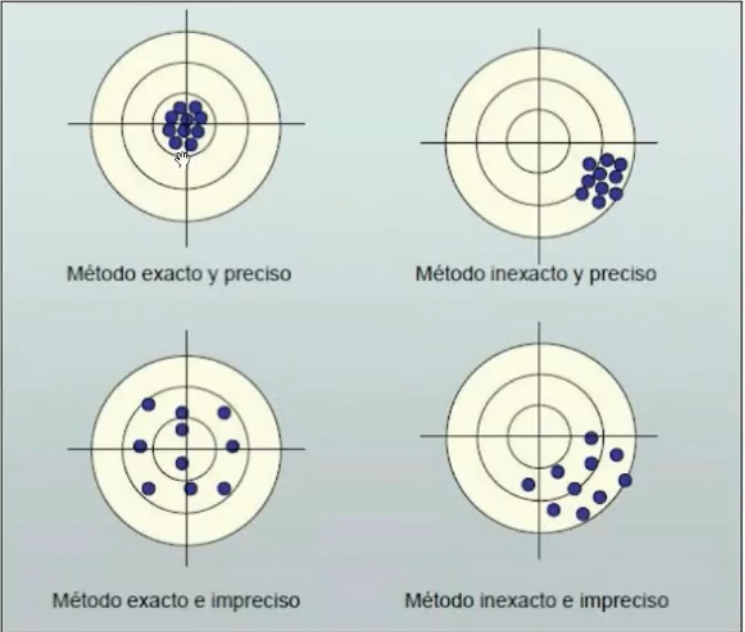
\includegraphics[width = 200px]{./img/tiro_al_blanco.png}
\end{itemize}

\subsection{Errores}

Valor aproximado entre un valor \textbf{real} y uno \textbf{proximo}.

\begin{equation}
	E = x_v - x_a
\end{equation}

Esto (1) se conoce como \textbf{error total}. En muchas ocaciones se trabaja
con el \textbf{error relativo} (2):

\begin{equation}
	E_r = \dfrac{x_v - x_a}{x_v}
\end{equation}

Y muchas otras veces se utiliza el \textbf{error relativo porcentual} (3):

\begin{equation}
	E_r = \dfrac{x_v - x_a}{x_v} 100%
\end{equation}

Muchos de los metodos son iterativos (Mejoran los resultados en cada iteracion). 
En la practica el valor \textbf{verdadero} no se conoce, por lo que se suele
trabajar con \textbf{errores aproximados} o aproximacion de errores.

\begin{equation}
	E_a = x_{actual} - x_{previo}
\end{equation}

\begin{equation}
	E_{ra} = \dfrac{x_{actual} - x_{previo}}{x_{actual}}
\end{equation}

\begin{equation}
	E_{ra}[\%] = \dfrac{x_{actual} - x_{previo}}{x_{actual}}100
\end{equation}

Si dichos errores aumentan con cada iteracion decimos que el metodo 
\textbf{diverge} a la solucion (El metodo no sirve para el problema elegido).
Sino, decimos que el metodo \textbf{converge} en la solucion

\pagebreak

\section{Raices de ecuaciones lineales}

\subsection{Presentacion del problema}

Para diversos problemas (Ej: amortiguacion de un auto) es muy utiliza
averiguar raices de ecuaciones.

\subsection{Metodo de la biseccion}

Este metodo sirve para todas las funciones excepto aquellas que tengan
\textbf{raices multiples de orden par}. Este metodo consiste en elegir 
\textbf{dos puntos} en una funcion continua y multiplicarlos Si hay un 
cambio de signo entonces en el intervalo entre ambos puntos 
\textbf{hay una raiz} (o mas de una).

\begin{equation}
	f(a)f(b) \leq 0
\end{equation}

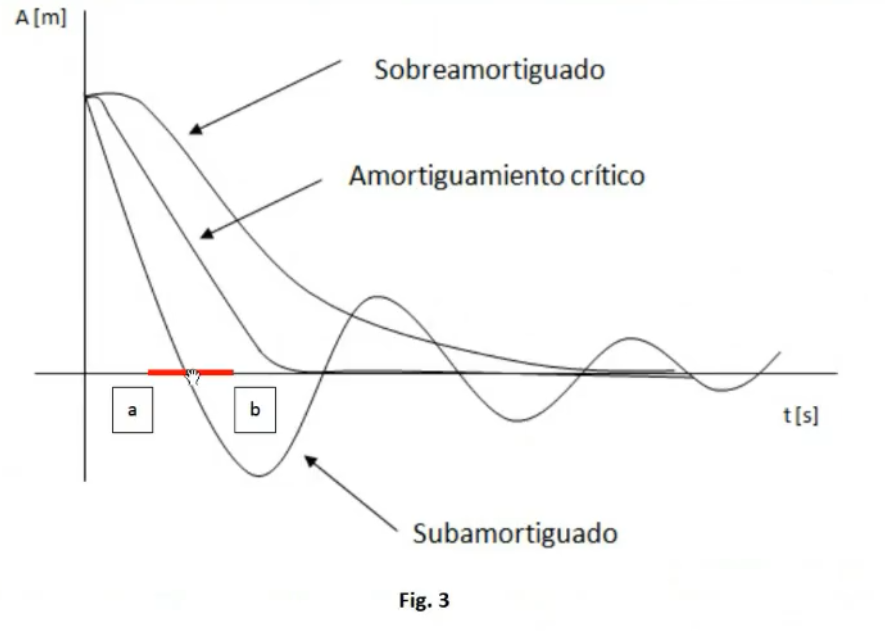
\includegraphics[width = 300px]{./img/biseccion.png}

Este metodo \textbf{no es util} cuando hay \textbf{muchas raices} 
en \textbf{intervalos muy pequeños}, ya que no nos dice la 
cantidad exacta de raices en el intervalo elegido.

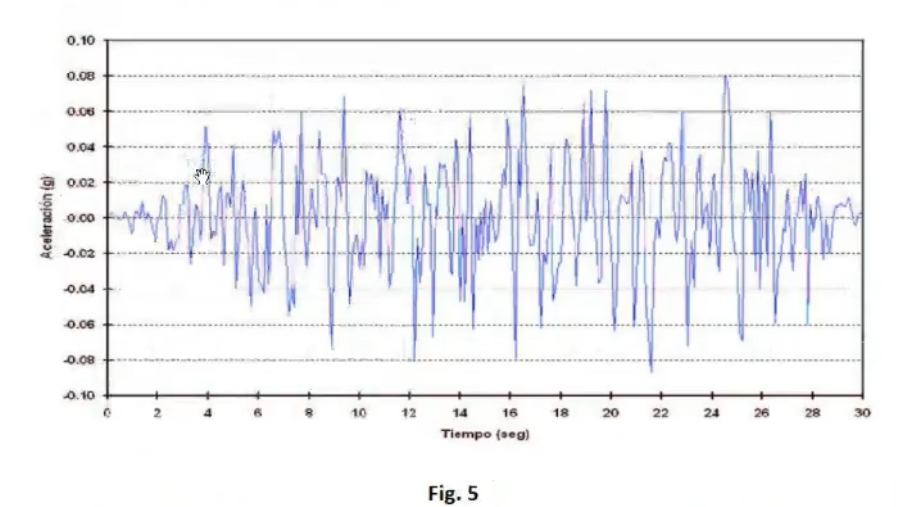
\includegraphics[width = 300px]{./img/sismo.png}

Para \textbf{calcular} la raiz de una funcion, se eligen los puntos
$a$ y $b$ y se aplica el metodo. Si hay una raiz, entonces se vuelve
a realizar el metodo pero en el intervalo $a$ y $c$ o $c$ y $a$ en 
donde c es:

\begin{equation}
	c = \dfrac{a+b}{2}
\end{equation}

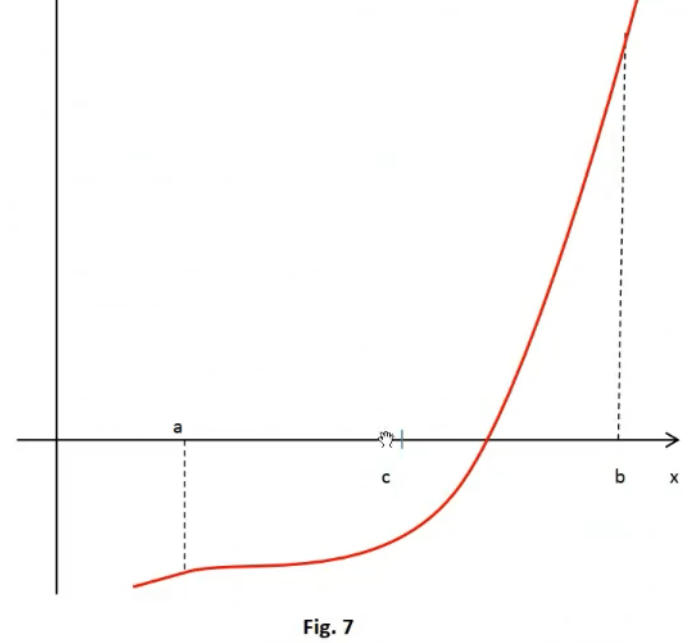
\includegraphics[width = 300px]{./img/biseccion_calcular.png}

Si $f(a)f(c) \leq 0$ entonces la raiz esta en el intervalo $a$ y 
$c$. sino, esta en el intervalo $c$ y $b$ 

\textbf{Ventajas de este metodo}

\begin{itemize}
	\item Alto grado de convergencia
	\item Confiable
	\item Facil programacion
\end{itemize}

\textbf{Desventajas}

\begin{itemize}
	\item No es apto para raices multiples de orden par
	\item convergencia \textbf{lenta}
\end{itemize}

\subsection{Metodo de punto fijo}

Este metodo coinciste en generar una funcion $g(x)$ a partir de la
funcion $f(x)$ original que intersecte a la funcion identidad.
De ser ese el caso, llamamos al punto interseccion punto fijo,
y en su dominio encontraremos la raiz de la funcion original.

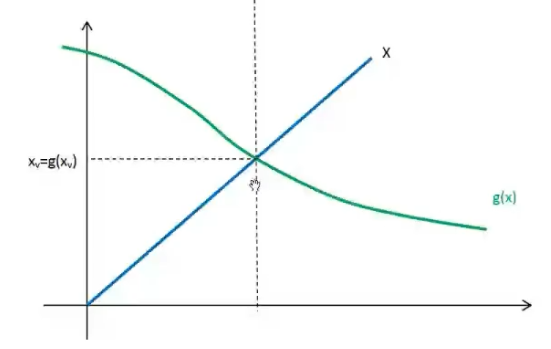
\includegraphics[width = 300px]{./img/punto_fijo.png}

\begin{equation}
	x_v = g(x_v)
\end{equation}

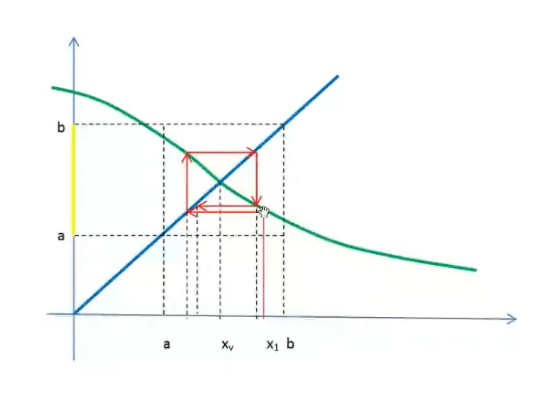
\includegraphics[width = 300px]{./img/punto_fijo_2.png}

Estas funciones $g(x)$ se obtienen de la funcion $f(x)$ original
de varias formas:

\begin{itemize}
	\item Por simple despeje
	\item Sumando o restando a ambos lados $x$ 
	\item Utilizando algun otro metodo matematico
	\item Proponiendo una $g(x)$ (Solo si se esta muy canchero)
\end{itemize}

No todas las funciones $g(x)$ funcionan, cuando no funcionan decimos
que son funciones \textbf{divergentes}. Para asegurarnos que la funcion
se comporte de manera \textbf{convergente}, esta debe cumplir con con 2 coindiciones:

\begin{enumerate}
	\item $g(x) \in [a, b]$ (amarillo)
	\item $|g'(\varepsilon)| \leq 1$ y $\varepsilon$ maximice la derivada
\end{enumerate}

Empezamos con $\varepsilon$ y aplicamos la formula:

\begin{equation}
	x_{i+1} = g(x_i)
\end{equation}

\textbf{Ventajas}

\begin{enumerate}
	\item Rapida convergencia
	\item Facil de programar
	\item Se puede partir de un valor proxmio sin importar de que lado esta la raiz (Metodo abierto)
\end{enumerate}

\textbf{Desventajas}

\begin{enumerate}
	\item Dificultad para encontrar una $g(x)$ convergente
	\item Puede quedar en un \textbf{lazo anidado}
\end{enumerate}

\subsection{Metodo de newton - raphson}

Este metodo se demuestra mediante procedimientos teoricos 
(\textbf{polinomio de Taylor}) y mediante procedimientos graficos.

\begin{equation}
	f(x_{i+1}) = f(x_i) + f'(x_i)(x_{i+1}-x_i) + \dfrac{f''(x_{i+1})}{2!}(x_{i+1}-x_i)^2 + \dots + \dfrac{f^n (x_{i+1})}{n!}(x_{i+1}-x_i)^n
\end{equation}

Lo que nosotros queremos es encontrar la raiz. por lo que queremos buscar
un $x$ tal que el polinomio de taylor de la funcion en cuestion de $0$.
Por lo que solo nos interesan los polinomios de taylor de orden 1 
(Generamos un \textbf{error de truncamiento}).

\begin{equation}
	f(x_{i+1}) = f(x_i) + f'(x_i)(x_{i+1} -x_i) = 0
\end{equation}

Despejando $x_{i+1}$ como nuestra supuesta raiz nos queda:

\begin{equation}
	x_{i+1} = x_i - \dfrac{f(x_i)}{f'(x_i)}
\end{equation}

Esto eso conoce como \textbf{formula recurrente del metodo Newton-Raphson}.

La interpretacion grafica consiste en ver la funcion (enfocandose en un punto) y su recta tangente, 
y mediante el triangulo rectangulo q se forma formulamos una ecuacion de la derivada de la funcion, 
en donde despejando $x_{i+1}$ nos quedaria $(13)$

Para llegar a la raiz, se aplica este función recursivamente

Este metodo es en realidad un subset del metodo de punto fijo, en donde:

\begin{equation}
	g(x_i) = x_i \dfrac{f(x_i)}{f'(x_i)}
\end{equation}

\textbf{Ventajas}
\begin{itemize}
	\item Alto grado de convergencia
	\item Metodo rapido y mas usado en la ingenieria
\end{itemize}

\textbf{Inconvenientes}
\begin{itemize}
	\item Problemas de convergencia en curvas planas (logaritmicas)
	\item En funciones complejas, encontrar la derivada puede ser muy dificil.
\end{itemize}

\subsection{Metodo de le secante}

Para cuando obtener la derivada se transforma en una tarea tediosa,
podemos mediante el teorema del \textbf{valor medio} sustituirla por
su aproximación (obteniendo un pequeño error)

\begin{equation}
	f'(x_i) = \dfrac{f(x_{i-1})-f(x_i)}{x_{i-1}-x_i}
\end{equation}

Reemplazando en Newton-Raphson:

\begin{equation}
	x_{i+1} = x_i - \dfrac{f(x_i)(x_{i-1}-x_i)}{f(x_{i-1})-f(x_i)}
\end{equation}

Usamos 2 puntos de partida, pero como es un metodo abierto, 
no importa si la raiz no esta entre esos 2 puntos.

La diferencia con el metodo anterior, es que en vez de utilizar
la recta tangente utilizamos la secante.

\pagebreak

\section{Sistemas de ecuaciones lineales}

\subsection{Presentación del problema}

Muchos problemas de la ingenieria en general se resuelven
al plantear y resolver un sitema de ecuaciones lineales.
En este capitulo vemos \textbf{solo} 3 metodos (hay muchos mas)

\subsection{Metodo de eliminación Gaussiana}

Dada una \textbf{matriz cuadrada} A, el metodo consiste en 2 pasos,
primero reducir esta matriz a una \textbf{triangular superior} mediante
operaciones elementales de filas, luego se realiza una \textbf{sustitución 
hacia atras} (despeje de los valores del vector X)

Nuestro problema consiste en resolver:

\begin{equation}
	A\overrightarrow{x} = \overrightarrow{b}
\end{equation}

No podes tener elementos nulos ni muy pequeños en la diagonal principal,
por lo que previamente tenemos que hacerla \textbf{diagonal principal dominante}
mediante operacion elemental tipo 3, o $E_{(ab)}$ 

Despeje de incognitas:

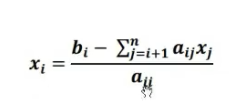
\includegraphics[width = 200px]{./img/secante_despeje.png}

La matriz puede estar bien o mal condicionada (lo vemos mas adelante)

\subsection{Metodo de Gauss - Seidel}

Metodo derivado de  Gauss Jacobi, pero mejorando la velocidad de convergencia.
Se basa en el principio del punto fijo.

De cada ecuación despejamos 1 incognita distinta, quedando ecuaciones de este tipo:

\begin{equation}
	x_1 = \dfrac{b_1 - a_{12}x_2 + a_{13}x_3 + \dots + a_{1n}x_n}{a_{11}}
\end{equation}

o

\begin{equation}
	x_i = \dfrac{b_i- \sum_{j=1}^n a_{ij}x_j}{a_{ii}}
\end{equation}

Donde $j \neq i$

\textbf{Nota}: no puede haber elementos nulos en la diagonal principal y
la matriz debe ser diagonal principal dominante.

Luego ed obtener estas funciónes, aplicamos el procedimiento del \textbf{punto fijo}
y obtenemos los valores para cada variable (al encontar un error permitido).

Este metodo produce mucha \textbf{Perdida de significancia}

\subsection{metodo de la LU}

Metodo muy utilizado en la ingenieria. Este metodo coinsiste en reemplazar

\begin{equation}
	[A][x] = [b]
\end{equation}

mediante propiedades algebraicas de matrices por:

\begin{equation}
	[LU][x] = [b]
\end{equation}

Donde L es una matriz triangular \textbf{inferior} (donde todos 
los elementos de la diagonal principal valen 1) y U \textbf{superior}.

o reemplazando:

\begin{equation}
	[L][y] = [b]
\end{equation}

Donde:

\begin{equation}
	[y] = [U][x]
\end{equation}

Para obtener las matrices L y U, aplicamos en metodo de eliminación Gaussiana,
en donde los elementos de L son los modificadores, y la matriz
U es la matriz triangulada por los mismos modificadores.


\pagebreak

\section{Ajuste de curvas}

\subsection{Presentacion del problema}

En muchas ocasiones en los problemas prácticos de la ingeniería, trabajamos con
datos experimentales discretos, es decir que obtenemos, por medición un conjunto de
puntos aislados que responden a una ley física específica. Por ende necesitaremos ajustar
curvas para interpolar valores entre los medidos para predecir el comportamiento del
fenómeno que estamos estudiando.
En este capítulo veremos varias formas de hacer esto, desde aproximar una simple
línea recta hasta un complejo polinomio trazador, pasando por la interpolación
polinomial.

\subsection{Regresion lineal por minimos cuadrados}

Es buscar una linea recta que pase lo mas cerca posible por todos los puntos, 
o dicho de otra manera que minimize los errores de aproximacion



\begin{equation}
	y = a_ + a_1x + E
\end{equation}

Donde $a_0$ y $a_1$ son la ordenada al origen y la pendiente respectivamente de la recta, 
y E es el error entre el modelo y las observaciones

La idea es minimizar la suma de todos los errores de todos los puntos:

\begin{equation}
	\sum_{i=1}^n E_i = \sum_{i=1}^n (y_i-a_0 - a_1x_i)
\end{equation}

Para que no haya ningun problema, se minimiza el cuadrado del error.

\begin{equation}
	S_r = \sum E_i^2
\end{equation}

Para encontrar las incognitas (terminos $a_0$ y $a_1$) derivamos respecto a esas incognitas:

\begin{equation}
	\dfrac{\partial S_r}{\partial a_0} =-2\sum (y_i-a_0-a_1x_i)
\end{equation}

\begin{equation}
	\dfrac{\partial S_r}{\partial a_1} =-2\sum [(y_i-a_0-a_1x_i)x_i]
\end{equation}

Que reescribiendo, formando un sistema de ecuaciones lineales, resolviendo y reordenando nos queda:

\begin{equation}
	a_1 = \dfrac{\sum x_i-y_1 - \sum x_i \sum y_i}{n\sum x_i^2 - (\sum x_i)^2}
\end{equation}

\begin{equation}
	a_0 = \overline{y} - a_i \overline{x}
\end{equation}

Este modelo es \textbf{lineal}. Pero no todas las curvas son rectas. Sin embargo, si son linealizables, se pueden resolver con este metodo aplicando 
algunos modelos no lineales. Algunos de estos son:

\textbf{Modelo exponencial}

Estas funciones son de la forma $ y = Ae^{Bx}$. Por lo que linearizando:

\begin{equation}
	a_0 = ln A
\end{equation}
	
\begin{equation}
	a_1 = B
\end{equation}

Por lo que cargariamos $(x_i, Ln (y_i))$

\textbf{Modelo potencial}

$Y = Ax^B$

cargariamos $(log x_i, Log y_1)$


Y deslinearizamos con:

\begin{equation}
	a_0 = Log A
\end{equation}

\begin{equation}
	a_1 = B
\end{equation}

\textbf{Modelo de crecimiento}

$y = A \dfrac{x}{b+x}$

cargariamos

Y deslinearizamos con:

\begin{equation}
	a_0 = \dfrac{1}{A}
\end{equation}

\begin{equation}
	a_1 = \dfrac{B}{A}
\end{equation}

\textbf{OJO QUE ALGUNAS FORMULAS ESTAN MAL, EDITAR!!!}

\subsection{Polinomio de Newton}

Antes, en la regrsion lineal, formabamos curvas que pasaran cerca de los puntos. Mediante Esta
interpolación, crearemos curvas que pasen por los puntos.

\subsection{Polinomio de Lagrange}

Reformulación del polinomio de Newton para no calcular 
las diferencias divididas. Este metodo tambien deriva del polinomio de Taylor,
obteniendose la siguiente expresión:

\begin{equation}
	f_n(x) = \sum_{i=0}^n L_i(x)f(x_i)
\end{equation}

Donde $L_i(x)$ son polinomios que cumplen con ciertas condiciones:

\begin{equation}
	L_i(x) = \Pi_{g=0}^n \dfrac{x-x_j}{x_i-x_j}
\end{equation}

Donde $j \neq i$



\end{document}